\documentclass[12 pt, a4paper]{article}
\usepackage[utf8]{inputenc}
\usepackage[letterpaper,top=2cm,bottom=2cm,left=3cm,right=3cm,marginparwidth=1.75cm]{geometry}
\usepackage[english, russian]{babel}
 \usepackage{graphicx}
 \usepackage{verbatim}

\title{Алгоритм Форчуна}
\author{Быкова Анна}
\date{Октябрь 2022}

\begin{document}

\maketitle

\section{Введение}
\subsection{Суть и назначение}
Алгоритм Форчуна – это алгоритм заметающей прямой для генерации диаграммы Вороного из набора точек на плоскости за время O(n log n) с использованием памяти O(n). Суль алгоритма в том, что он берет множесто 2D-точек, которые вводятся заранее и строит по ним диаграмму Вороного. Для каждой входной точки, которая называется «сайтом», нам нужно найти множество точек, которые ближе к этому месту, чем ко всем остальным. Такие множества точек образуют ячейки, множество которых и называется диаграммой Вороного.

суть алгоритма в следующем: по плоскости движется заметающая прямая (англ. sweepline). Движется скачками — от точки к точке. Первая часть этих точек — это точки со ввода, которые становятся сайтами. Вторая часть — это "виртуальные" точки, крайние по ходу движения заметающей прямой точки упомянутых описанных окружностей. При движении (параллельном переносе) заметающей прямой она касается любой такой описанной окружности дважды — второй раз эквивалентен событию, при котором диаграмма Вороного достраивается: к ней добавляется вершина, одно или более рёбер оканчиваются этой новой вершиной и одно или два новых ребра выходят из неё
\subsection{Авторство}
Данный алгоритм был опубликован Стивеном Форчуном в 1986 году в Нью Джерси во время Второго ежегодного симпозиума по Компьютерной Геометрии. Статья носит название «A Sweepline Algorithm for Voronoi Diagrams» . Название алгоритма происходит от имени его создателя.
\subsection{История развития}
Алгоритм увидел свет в 1986 году, в статье математика Стивена Форчуна под названием «Алгоритм развертки линий для диаграмм Вороного». Ни один из просмотренных источников не содержит более подробной информации об этом событии, о его предшественниках или об авторе, поэтому остановимся на этом.
\subsection{Состояние, реализация}
На момент своего появления, алгоритм Форчуна был первым в своем роде, который строил диаграмму Вороного с использованием заметающей прямой. Поскольку информация об этом алгоритме ограничена, можно сделать вывод, что он не сыскал популярности в свое время. Возможно это произошло из-за сложности вычислений, а модет и совсем по другим причинам.
\subsection{Перспектива Использования}
Алгоритм используется для построения диаграммы Вороного, которая в свою очередь имеет широкий спектр применения. 
Диаграммы Вороного постоянно использовались антропологами для описания регионов влияния различных культур; кристаллографами для объяснения структуры определенных кристаллов и металлов; экологами для изучения конкуренции между растениями; и экономистами для моделирования рынков в экономике США.Также, она используется в архитектуре, дизайне, поскольку образует красивые причудливые формы. 
\newpage
\section{Описание метода}
\subsection{Формальное}
Существует некоторое количество точек на плоскости - сайтов. Есть заметающая прямая, которая двигается (например) «сверху вниз», то есть от сайта с наибольшей ординатой к сайту с меньшей (от события к событию, если быть точным). Сразу стоит отметить, что влияние на построение диаграммы оказывают только те сайты, которые находятся выше или на заметающей прямой.
Когда ЗП попадает на очередной сайт (происходит событие точки (point event)), создаётся новая парабола (arch), фокусом которой является данный сайт, а директрисой — заметающая прямая. Эта парабола делит плоскость на две части — «внутренняя» область параболы соответствует точкам, которые сейчас ближе к сайту, а «внешняя» область — точкам, которые ближе к sweep line, ну а точки, лежащие на параболе — равноудалены от сайта и ЗП. Парабола будет меняться в зависимости от положения ЗП к сайту — чем дальше ЗП уходит от сайта вниз, тем больше расширяется парабола, однако в самом начале она вообще является отрезком («направленным» вверх). Далее парабола расширяется, у неё появляются две контрольные точки (break points) — точки её пересечения с остальными параболами («береговой линией»). В «береговой линии» мы храним дуги парабол от одной точки пересечения их друг с другом до другой, так и получается beach line. По сути, в этом алгоритме мы моделируем движение этой «береговой линии». потому как эти самые break point`ы движутся аккурат по рёбрам ячеек Вороного (ведь получается, что контрольные точки равноудалены от обоих сайтов, которым соответствуют эти параболы, да ещё и от ЗП).
И как раз-таки в тот момент, когда две контрольные точки — по одной из разных парабол — «встречаются», то есть как бы превращаются в одну, эта точка и становится вершиной ячейки Вороного (происходит событие круга (circle event)), причём в это время та дуга, которая находилась между этими двумя точками — «схлопывается» и удаляется из «береговой линии». Далее мы просто соединяем эту точку с предыдущей соответствующей ей и получаем ребро ячейки Вороного.

\newpage
\subsection{Математическое}
Оригинальный псевдокод алгоритма, описанный Стивеном Форчуном:\\
\begin{align}
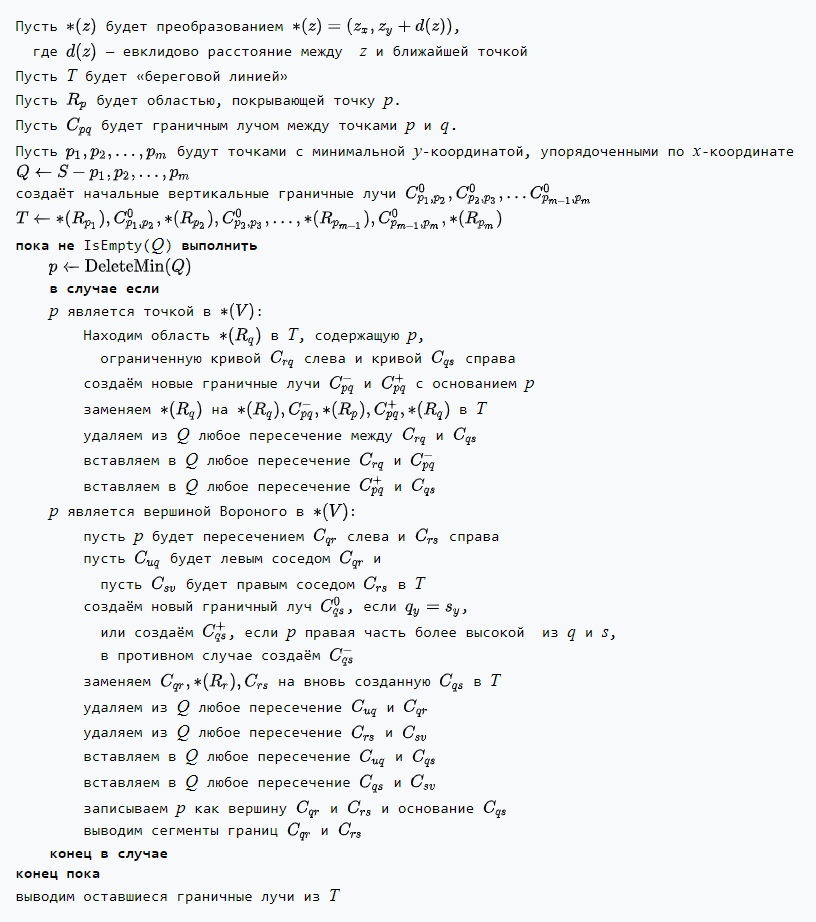
\includegraphics[scale = 0.55]{Псевдокод}
\end{center}
\newpage

\subsection{Пример}
Имеется поле с размерами: ширина – 1000, высота – 800. 
На ввод подаются 5 точек с координатами (208,235), (545,108), (342,601), (724,369), (455,352) соответственно. Программа считывает входные данные, располагает точки в местах, соответсвующих их координатам, проходит по ним сверху вниз заметающей прямой и строит диаграмму Вороного. Как результат работы алгоритма мы видим готовую диаграмму Вороного с простроенными ячейками, которая имеет подобный вид:\\
\begin{center}
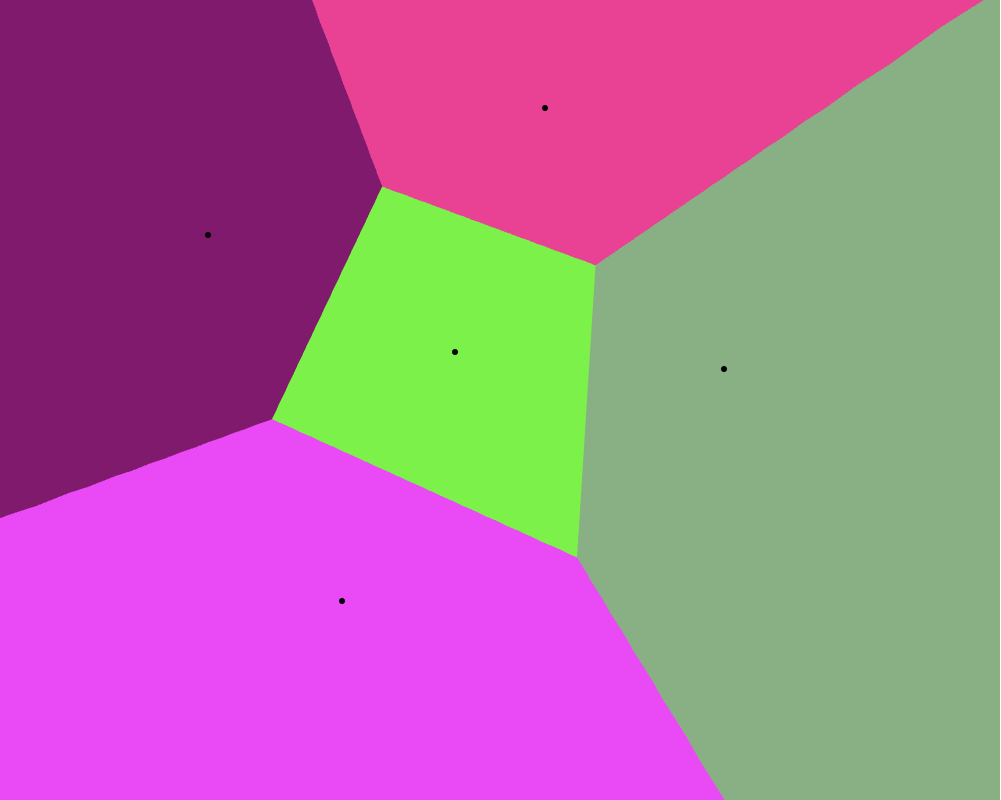
\includegraphics[scale = 0.4]{Диаграмма для задачи}
\end{center}
\newpage
\section{Формальная постановка задачи}
\subsection{Постановка задачи}
Написать программу, которая осуществляет построение диаграммы Вороного по алгоритму Форчуна. Пользователем в файл вводятся координаты точек плоскости (x, y - координаты), котореы считываются программой и преобразуются в готовую диаграмму Вороного, доступную в файле \textit{index.html}. Также, у пользователя должна быть возмоность динамически добавлять точки уже на готовой диаграмме с помощью левой клавиши мыши. При этом, программа дожна пересчитывать данные и выводить обновленный результат. 
\subsection{Формат входных данных}
Входной файл содержит координаты нескольких точек плоскости по которым следует построить диаграмму Вороного.
\subsection{Формат выходных данных}
При открытии файла \textit{index.html} должна быть выведена диаграмма Вороного.
\newpage
\section{Реализация}
\subsection{Point.js}
\begin{verbatim}
function Point(x, y){
	this.x = x;
	this.y = y;
}

Point.prototype.distance = function(a, b){
   return(Math.sqrt( (b.x-a.x)*(b.x-a.x) + (b.y-a.y)*(b.y-a.y) ));
}
\end{verbatim}
\subsection{VEdge.js}
\begin{verbatim}
function VEdge(s, a, b){		
	this.left = a;		
	this.right = b;		
	
	this.start = s;		
	this.end = null;	
	
	this.f = (b.x - a.x) / (a.y - b.y);
	this.g = s.y - this.f*s.x;
	this.direction = new Point(b.y-a.y, -(b.x - a.x));
	this.B = new Point(s.x+this.direction.x, s.y + this.direction.y);	
	
	this.intersected = false;
	this.iCounted = false;
	
	this.neighbour = null;
}
\end{verbatim}
\subsection{VEvent.js}
\begin{verbatim}
function VEvent(p, pe){
	this.point = p;
	this.pe = pe;
	this.y = p.y;
	this.key = Math.random()*100000000;
	
	this.arch = null;
	this.value = 0;
}

VEvent.prototype.compare = function(other){
	return((this.y>other.y)?1:-1);
}
\end{verbatim}
\subsection{VParabola.js}
\begin{verbatim}
function VParabola(s){
	this.cEvent = null;
	this.parent = null;
	this._left = null;
	this._right = null;
	
	this.site = s;
	this.isLeaf = (this.site != null);
}

VParabola.prototype = {
    get left(){
        return this._left;
    },
    get right(){
        return this._right;
    },
	
	set left(p){
        this._left = p;
		p.parent = this;
    },
    set right(p){
        this._right = p;
		p.parent = this;
    }
};
\end{verbatim}
\subsection{VPolygon.js}
\begin{verbatim}
function VPolygon(){
	this.size = 0;
	this.vertices = [];
	this.first = null;
	this.last = null;
}

VPolygon.prototype.addRight = function(p){
	this.vertices.push(p);
	++this.size;
	this.last = p;
	if(this.size==1) this.first = p;
}

VPolygon.prototype.addLeft  = function(p){
	var vs = this.vertices;
	this.vertices = [p];
	for(var i=0; i<vs.length; i++) 
		this.vertices.push(vs[i]);
		
	++this.size;
	this.first = p;
	if(this.size==1) this.last = p;
}
\end{verbatim}
\subsection{VQueue.js}
\begin{verbatim}
function VQueue(){
	this.q = new Array();
	this.i = 0;
}

function sortOnY(a, b){
	return (a.y > b.y)?1:-1 ;
}

VQueue.prototype.enqueue = function(p){
	this.q.push(p);
}

VQueue.prototype.dequeue = function(){
	this.q.sort(sortOnY);
	return this.q.pop();
}

VQueue.prototype.remove = function(e){
	var index = -1;
	for(this.i=0; this.i<this.q.length; this.i++)
	{
		if(this.q[this.i]==e){ index = this.i; break; }
	}
	this.q.splice(index, 1);
}

VQueue.prototype.isEmpty = function(){
	return (this.q.length==0);
}

VQueue.prototype.clear = function(b){
	this.q = [];
}
\end{verbatim}
\subsection{Voronoi.js}
\begin{verbatim}
function Voronoi(){
	with(this){
		this.places = null;
		this.edges = null;
		this.cells = null;
		this.queue = new VQueue;
		
		this.width = 0;
		this.heght = 0;
		this.root = null;
		this.ly = 0;
		this.lasty = 0;
		this.fp = null;
	}
}

Voronoi.prototype.Compute = function(p, width, height){
	if(p.length<2) return [];

	this.root = null;
	this.places = p;
	this.edges = [];
	this.cells = [];
	this.width = width;
	this.height = height;
	
	this.queue.clear(true);
	
	for(i=0; i<this.places.length; i++){
		var ev = new VEvent(this.places[i], true);
		var cell = new VPolygon();
		this.places[i].cell = cell;
		this.queue.enqueue(ev);
		this.cells.push(cell);
	}
	
	var lasty = Number.MAX_VALUE;
	var num = 0;
	while(!this.queue.isEmpty()){
		var e = this.queue.dequeue();  
		this.ly = e.point.y;
		if(e.pe) this.InsertParabola(e.point);
		else this.RemoveParabola(e);
		
		this.lasty = e.y;
	}
	this.FinishEdge(this.root);
	
	for(i=0; i<this.edges.length; i++)
		if(this.edges[i].neighbour) this.edges[i].start = this.edges[i].neighbour.end;
}

Voronoi.prototype.GetEdges = function(){
	return this.edges;
}

Voronoi.prototype.GetCells = function(){
	return this.cells;
}

		
Voronoi.prototype.InsertParabola = function(p){
	if(!this.root){this.root = new VParabola(p); this.fp = p; return;}
	
	if(this.root.isLeaf && this.root.site.y - p.y <0.01){	
		this.root.isLeaf = false;
		this.root.left = new VParabola(this.fp);
		this.root.right = new VParabola(p);
		var s = new Point((p.x+this.fp.x)/2, this.height);
		if(p.x>this.fp.x) this.root.edge = new VEdge(s, this.fp, p);
		else this.root.edge = new VEdge(s, p, this.fp);
		this.edges.push(this.root.edge);
		return;
	}
	
	var par = this.GetParabolaByX(p.x);
	
	if(par.cEvent){
		this.queue.remove(par.cEvent);
		par.cEvent = null;
	}

	var start = new Point(p.x, this.GetY(par.site, p.x));
	
	var el = new VEdge(start, par.site, p);
	var er = new VEdge(start, p, par.site);
	
	el.neighbour = er;
	this.edges.push(el);
	
	par.edge = er;
	par.isLeaf = false;
	
	var p0 = new VParabola(par.site);
	var p1 = new VParabola(p);
	var p2 = new VParabola(par.site);
	
	par.right = p2;
	par.left = new VParabola();
	par.left.edge = el;

	par.left.left = p0;
	par.left.right = p1;
	
	this.CheckCircle(p0);
	this.CheckCircle(p2);
}
		
Voronoi.prototype.RemoveParabola = function(e){		
	var p1 = e.arch;
	
	var xl = this.GetLeftParent(p1);
	var xr = this.GetRightParent(p1);
		
	var p0 = this.GetLeftChild(xl);
	var p2 = this.GetRightChild(xr);
	
	if(p0.cEvent){this.queue.remove(p0.cEvent); p0.cEvent = null;}
	if(p2.cEvent){this.queue.remove(p2.cEvent); p2.cEvent = null;}
				
	var p = new Point(e.point.x, this.GetY(p1.site, e.point.x));

	
	if(p0.site.cell.last == p1.site.cell.first ) p1.site.cell.addLeft(p);
	else p1.site.cell.addRight(p);
	
	p0.site.cell.addRight(p);
	p2.site.cell.addLeft(p);
	
	this.lasty = e.point.y;
		
	xl.edge.end = p;
	xr.edge.end = p;
	
	var higher;
	var par = p1;
	while(par != this.root){
		par = par.parent;
		if(par == xl) {higher = xl;}
		if(par == xr) {higher = xr;}
	}
	
	higher.edge = new VEdge(p, p0.site, p2.site);

	this.edges.push(higher.edge);
	
	var gparent = p1.parent.parent;
	if(p1.parent.left == p1){
		if(gparent.left  == p1.parent) gparent.left  = p1.parent.right;
		else p1.parent.parent.right = p1.parent.right;
	}
	else{
		if(gparent.left  == p1.parent) gparent.left  = p1.parent.left;
		else gparent.right = p1.parent.left;
	}
	
	this.CheckCircle(p0);
	this.CheckCircle(p2)
}

Voronoi.prototype.FinishEdge = function(n){
	var mx;
	if(n.edge.direction.x > 0.0)
	{
		mx = Math.max(this.width, n.edge.start.x + 10 );
	}
	else
	{
		mx = Math.min(0.0, n.edge.start.x - 10);
	}
	n.edge.end = new Point(mx, n.edge.f*mx + n.edge.g);
	
	if(!n.left.isLeaf)  this.FinishEdge(n.left);
	if(!n.right.isLeaf) this.FinishEdge(n.right);
}

Voronoi.prototype.GetXOfEdge = function(par, y) {

	var left =	this.GetLeftChild (par);
	var right =	this.GetRightChild(par);
			
	var p = left.site;
	var r = right.site;
	
	var dp = 2*(p.y - y);
	var a1 = 1/dp;
	var b1 = -2*p.x/dp;
	var c1 = y+dp*0.25 + p.x*p.x/dp;
	
	dp = 2*(r.y - y);
	var a2 = 1/dp;
	var b2 = -2*r.x/dp;
	var c2 = y+dp*0.25 + r.x*r.x/dp;
	
	var a = a1 - a2;
	var b = b1 - b2;
	var c = c1 - c2;
	
	if(a==0) return -c/b;
	
	var disc = b*b - 4 * a * c;
	var x1 = (-b + Math.sqrt(disc)) / (2*a);
	var x2 = (-b - Math.sqrt(disc)) / (2*a);

	var ry;
	if(p.y < r.y ) ry =  Math.max(x1, x2);
	else ry = Math.min(x1, x2);
	
	return ry;
}

Voronoi.prototype.GetParabolaByX = function(xx){
	var par = this.root;
	var x = 0;
	
	while(!par.isLeaf)
	{
		x = this.GetXOfEdge(par, this.ly);
		if(x>xx) par = par.left;
		else par = par.right;				
	}
	return par;
}

Voronoi.prototype.GetY = function(p, x) {
	var dp = 2*(p.y - this.ly);
	var b1 = -2*p.x/dp;
	var c1 = this.ly+dp/4 + p.x*p.x/dp;
	
	return(x*x/dp + b1*x + c1);
}

Voronoi.prototype.CheckCircle = function(b){
	var lp = this.GetLeftParent(b);
	var rp = this.GetRightParent(b);
	
	var a = this.GetLeftChild(lp);
	var c = this.GetRightChild(rp);
	
	if(!a || !c || a.site == c.site) return;
	
	var s = this.GetEdgeIntersection(lp.edge, rp.edge);
	if(!s) return;
	
	var d = Point.prototype.distance(a.site, s);
	//if(d > 5000) return;
	if(s.y - d  >= this.ly) return;
	
	var e = new VEvent(new Point(s.x, s.y - d), false);
	
	b.cEvent = e;
	e.arch = b;
	this.queue.enqueue(e);
}

Voronoi.prototype.GetEdgeIntersection = function(a, b){
	var I = GetLineIntersection(a.start, a.B, b.start, b.B);
	
	var wd = 	(I.x - a.start.x)*a.direction.x<0 || (I.y - a.start.y)*a.direction.y<0	
			 ||	(I.x - b.start.x)*b.direction.x<0 || (I.y - b.start.y)*b.direction.y<0;	
			 
	if(wd) return null;
	return I;
}

Voronoi.prototype.GetLeft = function(n){
	return this.GetLeftChild( this.GetLeftParent(n));
}
		
Voronoi.prototype.GetRight = function(n){
	return this.GetRightChild(this.GetRightParent(n));
}	
		
Voronoi.prototype.GetLeftParent = function(n){
	var par = n.parent;
	var pLast = n;
	while(par.left == pLast) 
	{ 
		if(!par.parent) return null;
		pLast = par; par = par.parent; 
	}
	return par;
}

Voronoi.prototype.GetRightParent = function(n){
	var par = n.parent;
	var pLast = n;
	while(par.right == pLast) 
	{	
		if(!par.parent) return null;
		pLast = par; par = par.parent;	
	}
	return par;
}

Voronoi.prototype.GetLeftChild = function(n){
	if(!n) return null;
	var par = n.left;
	while(!par.isLeaf) par = par.right;
	return par;
}

Voronoi.prototype.GetRightChild = function(n){
	if(!n) return null;
	var par = n.right;
	while(!par.isLeaf) par = par.left;
	return par;
}

function GetLineIntersection(a1, a2, b1, b2){
	var dax = (a1.x-a2.x), dbx = (b1.x-b2.x);
	var day = (a1.y-a2.y), dby = (b1.y-b2.y);
			
	var Den = dax*dby - day*dbx;
	if (Den == 0) return null;	// parallel

	var A = (a1.x * a2.y - a1.y * a2.x);
	var B = (b1.x * b2.y - b1.y * b2.x);
		
	var I = new Point(0,0);
	I.x = ( A*dbx - dax*B ) / Den;
	I.y = ( A*dby - day*B ) / Den;
	
	return I;
}
\end{verbatim}
\subsection{index.html}
\begin{verbatim}
<html> 
	<head> 
		<title>Voronoi diagram</title> 
		<meta charset="utf-8" /> 
		<style type="text/css">
			body { margin: 0; padding: 0; height: 100%; font-size:20px;}
		</style>
		
		<script type="text/javascript" src="Point.js"></script> 
		<script type="text/javascript" src="VEdge.js"></script> 
		<script type="text/javascript" src="VEvent.js"></script> 
		<script type="text/javascript" src="VParabola.js"></script> 
		<script type="text/javascript" src="VQueue.js"></script>
		<script type="text/javascript" src="VPolygon.js"></script>
		<script type="text/javascript" src="Voronoi.js"></script> 
		
		<script type="application/javascript">
			var voronoi = true;
			var delaunay = false;
			var canv = null;
			var colors = [];
			
			function mouseX(e){	return e.clientX - e.target.offsetLeft;}
			function mouseY(e){	return e.clientY - e.target.offsetTop; }
			
			function onLoad()
			{
				canv = document.getElementById("c");
				canv.onmousemove = onMM;
				canv.onclick = onClick;
				c = canv.getContext("2d");
				w = canv.width = window.innerWidth;
				h = canv.height = window.innerHeight;
				points = [];
				v = new Voronoi();
				
				for(i=0; i<5; i++)
				{
					points.push(new Point(Math.random()*w, Math.random()*h));
					colors.push(rndCol());
				}
					
				redraw();
			}
			
			function onMM(e)
			{
				var last = points[points.length-1];
				last.x = mouseX(e);
				last.y = mouseY(e);
				redraw();
			}
			
			function onClick(e)
			{
				var last = points[points.length-1];
				last.x += Math.random();
				last.y += Math.random();
				points.push( new Point(mouseX(e), mouseY(e)));
				colors.push(rndCol());
			}
			function resetPoints()
			{
				points = [points[points.length-1]];
				redraw();
			}
			
			function redraw()
			{
				c.fillStyle = "#ffffff";
				c.fillRect (0, 0, w, h);
				
				v.Compute(points, w, h);
				edges = v.GetEdges();
				cells = v.GetCells();
				

				c.lineWidth = 5;
				c.strokeStyle = "#000";
				for(i=0; i<edges.length; i++)
				{
					var e = edges[i];
					c.beginPath();
					c.moveTo(e.start.x, e.start.y);
					c.lineTo(e.end.x, e.end.y);
					c.closePath();
					c.stroke();
				}

				
				c.fillStyle = "rgb(0,255,0)";
				for(i=0; i<points.length; i++)
				{
					var p = points[i];
					c.beginPath();
					c.arc(p.x, p.y, 6, 0, Math.PI*2, true);
					c.closePath();
					c.fill();
				}
			}
			function rndCol() {
				var letters = '0123456789ABCDEF'.split('');
				var color = '#';
				for (var i = 0; i < 6; i++ ) {
					color += letters[Math.round(Math.random() * 15)];
				}
				return color;
			}
		</script> 
	</head> 
	
	<body onload="onLoad()" > 
		<form style="position:absolute; z-index:1; margin:10px">
			<input type="button" value="Сброс" onclick="resetPoints();" style="width:100px; height:30px;"/>
		</form>
		<canvas id="c"> </canvas>
	</body> 
</html>
\end{verbatim}
\section{Список литературы}
\begin{enumerate}
\item Steven Fortune. A sweepline algorithm for Voronoi diagrams // ACM Digital Library Proceedings of the second annual symposium on Computational geometry. — Yorktown Heights, New York, United States, 1986. — ISBN 0-89791-194-6. 
\item Mark de Berg, Marc van Kreveld, Mark Overmars, Otfried Schwarzkopf. Computational Geometry. — 2nd revised. — Springer-Verlag, 2000. — ISBN 3-540-65620-0.
\item David Austin. Voronoi Diagrams and a Day at the Beach. — American Mathematical Society.
\item Rene Descartes, Le Monde, ou Traité de la lumière, Translation and introduction by M.S. Mahoney, Abaris, 1979.
\item A. Okabe, B. Boots, K. Sugihara, S. Chiu, Spatial Tesselations, Concepts and Applications of Voronoi Diagrams, Wiley, 2000.
\item J. O'Rourke, Computational Geometry in C, Cambridge University Press, 2000.
\item Spatial: диаграмма Вороного (Java) [Электронный ресурс] — Режим доступа: http://obi2ru.blogspot.com/2012/12/spatial-voronoi-diagram-by-java.html
\item Kenny Wong, Hausi A. Müller, An Efficient Implementation of Fortune's Plane-Sweep Algorithm for Voronoi Diagrams, CiteSeerX   10.1.1.83.5571 .
\item Wikipedia: Алгоритм Форчуна 
\item Javascript Implementation of Steven J. Fortune's Algorythm to compute Voronoi diagrams [Электронный ресус] — Режим доступа: http://www.raymondhill.net/voronoi/rhill-voronoi.html
\item Алгоритм Форчуна, подробности реализации [Электронный ресус] — Режим доступа: https://habr.com/ru/post/430628/
\item Ход «Voronoi» [Электронный ресус] — Режим доступа: https://habr.com/ru/post/110790/
\item Ход «Voronoi». Часть 2 — Бинарное дерево  [Электронный ресус] — Режим доступа: https://habr.com/ru/post/112581/
\item С++ для начинающих. Бинарное дерево. Первое знакомство [Электронный ресус] — Режим доступа: https://ci-plus-plus-snachala.ru/?p=89
\item Практика метапрограммирования на C++: бинарное дерево поиска на этапе компиляции [Электронный ресус] — Режим доступа: https://habr.com/ru/p ost/320686/
\item Fortune's Algorithm in C++ [Электронный ресус] — Режим доступа: https://www.cs.hmc.edu/-mbrubeck/voronoi.html
\item Voronoi diagrams with Fortune's algorithm  [Электронный ресус] — Режим доступа: https://www.bitbanging.space/posts/voronoi-diagram-with-fortunes-algorithm
\item Wikipedia: Fortune's algorithm
\item Fortune's algorithm  [Электронный ресус] — Режим доступа: https://wikimili.com/en/Fortune's-algorithm
\item Диаграмма Вороного и её применения [Электронный ресус] — Режим доступа: https://itnan.ru/post.php?c=1&p=309252
\item Voronoi Diagrams and a Day at the Beach [Электронный ресус] — Режим доступа: https://www.ams.org/publicoutreach/feature-column/fcarc-voronoi
\item Voronoi diagram in AS3 [Электронный ресус] — Режим доступа: https://blog.ivank.net/voronoi-diagram-in-as3.html
\item Алгоритм Форчуна на C++ для построения диаграммы Вороного на плоскости [Электронный ресус] — Режим доступа: https://www.pvsm.ru/matematika/211589
\item THE BOOST.POLYGON VORONOI LIBRARY [Электронный ресус] — Режим доступа: https://www.boost.org/doc/libs/1-52-0/libs/polygon/doc/voronoi-main.htm
\item Voronoi Diagram using Fortune's Algorithm [Электронный ресус] — Режим доступа: https://www.youtube.com/watch?v=dgEt9Go7GvE
\item Voronoi Diagrams and Procedural Map Generation [Электронный ресус] — Режим доступа: https://www.youtube.com/watch?v=3G5d8ob-Lfo
\item Fortune's Algorithm: The Details [Электронный ресус] — Режим доступа: https://pvigier.github.io/2018/11/18/fortune-algorithm-details.html
\end{enumerate}

\end{document}